\documentclass[9pt,conference]{IEEEtran}
\usepackage[english]{babel}
\usepackage[utf8]{inputenc}
\usepackage{amssymb}
\usepackage{amsmath}
\usepackage{cases}
\usepackage{booktabs}
\usepackage{graphicx}

\usepackage[bottom]{footmisc}

% Format
\usepackage{anysize}
\usepackage[a4paper, top=20mm, bottom=20mm, left=15mm, right=15mm]{geometry}
\columnsep 4mm
% \linespread{0.95}
% \usepackage[a4paper, top=29mm, bottom=30mm, left=15mm, right=15mm]{geometry}
% \columnsep 5mm
% \linespread{1}

% Balance the columns on the last page
\usepackage{flushend}

% Bibliography
\usepackage{csquotes}
\usepackage[backend=biber, maxnames=1, sorting=none]{biblatex}
\renewcommand*{\bibfont}{\small}

% Text
\newcommand{\qoi}{QOI}
\newcommand{\qois}{QOIs}

\newcommand{\qom}{QOM}
\newcommand{\qoms}{QOMs}

\newcommand{\ie}{\emph{i.e.}}
\newcommand{\eg}{\emph{e.g.}}
\newcommand{\etc}{\emph{etc.}}
\newcommand{\perse}{\emph{per se}}

\makeatletter
\def\stage#1{\@ifnextchar\bgroup{\stageDouble{#1}}{\stageSingle{#1}}}
\def\stageSingle#1{Stage~#1}
\def\stageDouble#1#2{Stage~#1.\hspace{0.5em}\emph{#2}}
\makeatother

\newcommand{\blindreview}{%
  \textnormal{%
    $\text{HIDDEN FOR BLIND REVIEW}$%
  }%
}

\usepackage{array}
\newcolumntype{=}{>{\global\let\currentrowstyle\relax}}
\newcolumntype{-}{>{\currentrowstyle}}
\newcommand{\rowstyle}[1]{\gdef\currentrowstyle{#1}%
  #1\ignorespaces
}

% Tables and figures
\setlength{\topsep}{0pt}
\setlength{\abovecaptionskip}{5pt}
\setlength{\belowcaptionskip}{0pt}
\renewcommand{\arraystretch}{1.0}
\setlength{\tabcolsep}{4pt}

% Formulas
\setlength\abovedisplayskip{5pt}
\setlength\belowdisplayskip{5pt}

% References
\newcommand{\eref}[1]{Eq.~(\ref{equ:#1})}
\newcommand{\sref}[1]{Sec.~\ref{sec:#1}}
\newcommand{\aref}[1]{Appendix~\ref{app:#1}}
\newcommand{\fref}[1]{Fig.~\ref{fig:#1}}
\newcommand{\tref}[1]{Tab.~\ref{tab:#1}}

\newcommand{\elabel}[1]{\label{equ:#1}}
\newcommand{\slabel}[1]{\label{sec:#1}}
\newcommand{\alabel}[1]{\label{app:#1}}
\newcommand{\flabel}[1]{\label{fig:#1}}
\newcommand{\tlabel}[1]{\label{tab:#1}}

% Sets
\newcommand{\real}{\mathbb{R}}

% Linear algebra
\newcommand{\m}[1]{\mathbf{#1}}
\renewcommand{\v}[1]{\mathbf{#1}}

\newcommand{\abs}[1]{| #1 |}
\newcommand{\norm}[1]{\| #1 \|}

\newcommand{\vI}{\v{e}}
\newcommand{\mI}{\m{I}}
\newcommand{\mOne}{\m{I}}
\newcommand{\vZero}{\v{0}}

\newcommand{\diag}[1]{\text{diag}(#1)}

% Probability theory
\renewcommand{\o}{\omega}
\newcommand{\outcomes}{\Omega}
\newcommand{\sigmaAlgebra}{\mathcal{F}}
\newcommand{\probabilityMeasure}{\mathbb{P}}
\newcommand{\probabilitySpace}{(\outcomes, \sigmaAlgebra, \probabilityMeasure)}

\newcommand{\gaussian}[2]{\mathcal{N}\left( #1, #2 \right)}
\newcommand{\gaussianp}[2]{\mathcal{GP}\left( #1, #2 \right)}
\newcommand{\sichisquared}[2]{\text{Scale-inv-}\chi^2\left( #1, #2 \right)}
\newcommand{\studentst}[3]{t_{#1}\left( #2, #3 \right)}

\makeatletter
\def\f#1{\@ifnextchar\bgroup{\fWithTwoArguments{#1}}{\fWithOneArgument{#1}}}
\def\fWithTwoArguments#1#2{p_{#1}( #2 )}
\def\fWithOneArgument#1{p( #1 )}

\def\fMean{\@ifnextchar\bgroup{\fMeanWithArgument}{\fMeanWithoutArgument}}
\def\fMeanWithArgument#1{\mu(#1)}
\def\fMeanWithoutArgument{\mu}

\def\fCov{\@ifnextchar\bgroup{\fCovWithArgument}{\fCovWithoutArgument}}
\def\fCovWithArgument#1{k(#1)}
\def\fCovWithoutArgument{k}

\def\E{\@ifnextchar\bgroup{\EWithArgument}{\EWithoutArgument}}
\def\EWithArgument#1{\mathbb{E}\left( #1 \right)}
\def\EWithoutArgument{\mathbb{E}}
\makeatother

\newcommand{\Cov}[1]{\mathbb{C}\text{ov}\left( #1 \right)}

\newcommand{\mCov}{\m{K}}

\newcommand{\mean}{\mu}
\newcommand{\vmean}{{\boldsymbol\mu}}

% Karhunen-Loeve expansion
\newcommand{\domain}{\mathcal{R}}
\newcommand{\mKL}{\m{L}}

% Temperature
\newcommand{\T}{q}
\newcommand{\vT}{\v{q}}
\newcommand{\mT}{\m{Q}}
\newcommand{\mvT}{\v{q}}
\newcommand{\amb}{\text{amb}}
\newcommand{\meas}{\text{msr}}

% Power
\newcommand{\p}{p}
\renewcommand{\P}{p}
\newcommand{\vP}{\v{p}}
\newcommand{\mP}{\m{P}}
\newcommand{\dyn}{\text{dyn}}
\newcommand{\leak}{\text{leak}}

% Thermal model
\renewcommand{\t}{t}

\newcommand{\specification}{\mathcal{S}}

\newcommand{\vX}{\v{x}}
\newcommand{\mC}{\m{C}}
\newcommand{\mG}{\m{G}}
\newcommand{\mM}{\m{B}}

% Data model
\renewcommand{\r}{r}
\newcommand{\vr}{\v{r}}

% Quantity of interest
\renewcommand{\u}{u}
\newcommand{\vu}{\v{u}}
\newcommand{\mU}{\m{U}}

% Quantity of measure
\newcommand{\q}{q}
\newcommand{\vq}{\v{q}}
\newcommand{\mQ}{\m{Q}}

\makeatletter
\def\oBB{\@ifnextchar\bgroup{\oBBPlus}{\oBBZero}}
\def\oBBPlus#1{\@ifnextchar\bgroup{\oBBTwo{#1}}{\oBBOne{#1}}}
\def\oBBTwo#1#2{f_{#1}\left(#2\right)}
\def\oBBOne#1{f\left(#1\right)}
\def\oBBZero{f}
\makeatother

% Statistical model
\newcommand{\QData}{\mathcal{Q}}
\newcommand{\UData}{\mathcal{U}}

\newcommand{\noise}{\epsilon}
\newcommand{\mnoise}{\boldsymbol\epsilon}
\newcommand{\vnoise}{\boldsymbol\epsilon}

\newcommand{\z}{z}
\newcommand{\vz}{\v{z}}

\newcommand{\param}{\theta}
\newcommand{\Param}{\Theta}

\newcommand{\vparam}{{\boldsymbol\theta}}

\newcommand{\SE}{\text{SE}}
\newcommand{\OU}{\text{OU}}

\newcommand{\mOI}{\m{J}}

% Profiles
\newcommand{\profile}[1]{( #1, \partition{#1} )}

\newcommand{\partition}[1]{\tau[#1]}

\makeatletter
\def\profileP{\@ifnextchar\bgroup{\profilePWithArgument}{\profilePWithoutArgument}}
\def\profilePWithArgument#1{\profile{\mP(#1)}}
\def\profilePWithoutArgument{\profile{\mP}}

\newcommand{\profilePdyn}{(\mP_\dyn, \partition{\mP})}

\def\profileT{\@ifnextchar\bgroup{\profileTWithArgument}{\profileTWithoutArgument}}
\def\profileTWithArgument#1{\profile{\mT(#1)}}
\def\profileTWithoutArgument{\profile{\mT}}
\makeatother

% Numbers
\newcommand{\ndies}{{n_\text{d}}}
\newcommand{\nrdies}{{n_\text{d}'}}

\newcommand{\nprocs}{{n_\text{p}}}
\newcommand{\nrprocs}{{n_\text{p}'}}

\newcommand{\nsteps}{{n_\text{t}}}
\newcommand{\nrsteps}{{n_\text{t}'}}

\newcommand{\nnodes}{{n_\text{n}}}
\newcommand{\nvars}{{n_\text{v}}}

\newcommand{\nsamples}{{n_\text{mc}}}


\bibliography{include/references.bib}

\begin{document}
  \title{Statistical Analysis of Process Variation Based on Indirect Measurements for Electronic System Design}

  \author{
    \IEEEauthorblockN{Ivan Ukhov}
\IEEEauthorblockA{Link\"{o}ping University\\Sweden\\ivan.ukhov@liu.se}
\and
\IEEEauthorblockN{Mattias Villani}
\IEEEauthorblockA{Link\"{o}ping University\\Sweden\\mattias.villani@liu.se}
\and
\IEEEauthorblockN{Petru Eles}
\IEEEauthorblockA{Link\"{o}ping University\\Sweden\\petru.eles@liu.se}
\and
\IEEEauthorblockN{Zebo Peng}
\IEEEauthorblockA{Link\"{o}ping University\\Sweden\\zebo.peng@liu.se}

  }

  \maketitle

  \begin{abstract}
    In this paper, we propose and develop a novel multiprocessor system design framework for the analysis of process variations across semiconductor wafers. Instead of taking direct measurements of the quantity of interest being characterized, our technique operates on indirect observations, namely, on temperature profiles, which are cheap to collect as no deployment of expensive test structures is required.
The experimental results provide a comprehensive study of our approach for a wide range of configurations having high practical importance.

  \end{abstract}

  \section{Introduction and Prior Work} \slabel{introduction}
  Process variation constitutes one of the major concerns of electric system designs \cite{chandrakasan2001, srivastava2010}. A crucial implication of process variation is that it renders the key parameters of a technological process, \eg, the effective channel length, gate oxide thickness, and threshold voltage, as uncertain quantities.
Therefore, the same workload applied to two ``identical'' dies can lead to two different power and, thus, temperature profiles since they essentially depend on those stochastic quantities.
Consequently, process variation leads to performance degradation in the best case and to burnt silicon in the worst scenario.
Under these circumstances, uncertainty quantification has evolved into an indispensable asset of the fabrication workflows that can provide high guaranties on the efficiency and robustness of their products.

An important target of uncertainty quantification is the characterization of the on-wafer distribution of a quantity of interest (\qoi), deteriorated by process variation, based on a data set of measurements.
The problem belongs to the class of so-called inverse problems since the \qoi\ can be seen as an input and the measurements as an output, which is opposed to direct problems wherein one studies outputs based on the knowledge of inputs (see, \eg, \cite{juan2011, juan2012}).
Such an inverse problem is addressed in this paper: our goal is to quantify distributions of the key process parameters, \eg, the effective channel length, and we approach this goal by measuring temperature and analyzing it via the machinery of Bayesian inference \cite{gelman2004}.

Bayesian inference is utilized in \cite{zhang2010} to identify an optimal set of locations on the wafer, in which the \qois\ should be measured in order to characterize them with the maximal accuracy.
In \cite{paek2012}, the authors consider an inverse problem focused on the inference of the power dissipation based on transient temperature profiles using Markov random fields.
Another temperature-based characterization of power is developed in \cite{mesa-martinez2007} wherein a genetic algorithm is employed for reconstruction of the power model.
It should be noted that the approach in \cite{zhang2010} requires test structures to be deployed onto each die on the wafer as it operates on direct measurements, which can be expensive and, thus, impractical to undertake. Moreover, the technique in \cite{zhang2010}, focusing on frequencies, voltages, and currents, is not capable of characterizing the primary sources of uncertainty such as the effective channel length and gate oxide thickness since it would require the measured dies to be destroyed. The approaches in \cite{paek2012} and \cite{mesa-martinez2007}, on the other hand, solving the inverse temperature-to-power problem, are not aware of process variation.

Our work makes the following main contributions. First, we propose a novel approach to the quantification of process variation based on a data set of indirect, incomplete, and noisy measurements. Indirectness is the key ingredient as it allows for a significant decrease of the costs associated with the process variation characterization. Second, we develop a solid framework around the proposed idea in order to make the method readily available for practical implementations. Third, we present a thorough study of various aspects of the framework that are of high practical interests.

The remainder of the paper is organized as follows. A motivational example is given in \sref{motivation}. In \sref{problem-formulation}, we formulate the problem, which we address, and state our solution. Preliminary materials on Bayesian inference are given in \sref{preliminaries}. The proposed framework is presented in \sref{proposed-framework}, which is followed by the experimental results reported in \sref{experimental-results}. \sref{conclusion} concludes the paper. The work also includes a set of supplementary materials given in the appendix.


  \section{Motivational Example} \slabel{motivation}
  \begin{figure}[b!]
  \vspace{-1.5em}
  \centering
  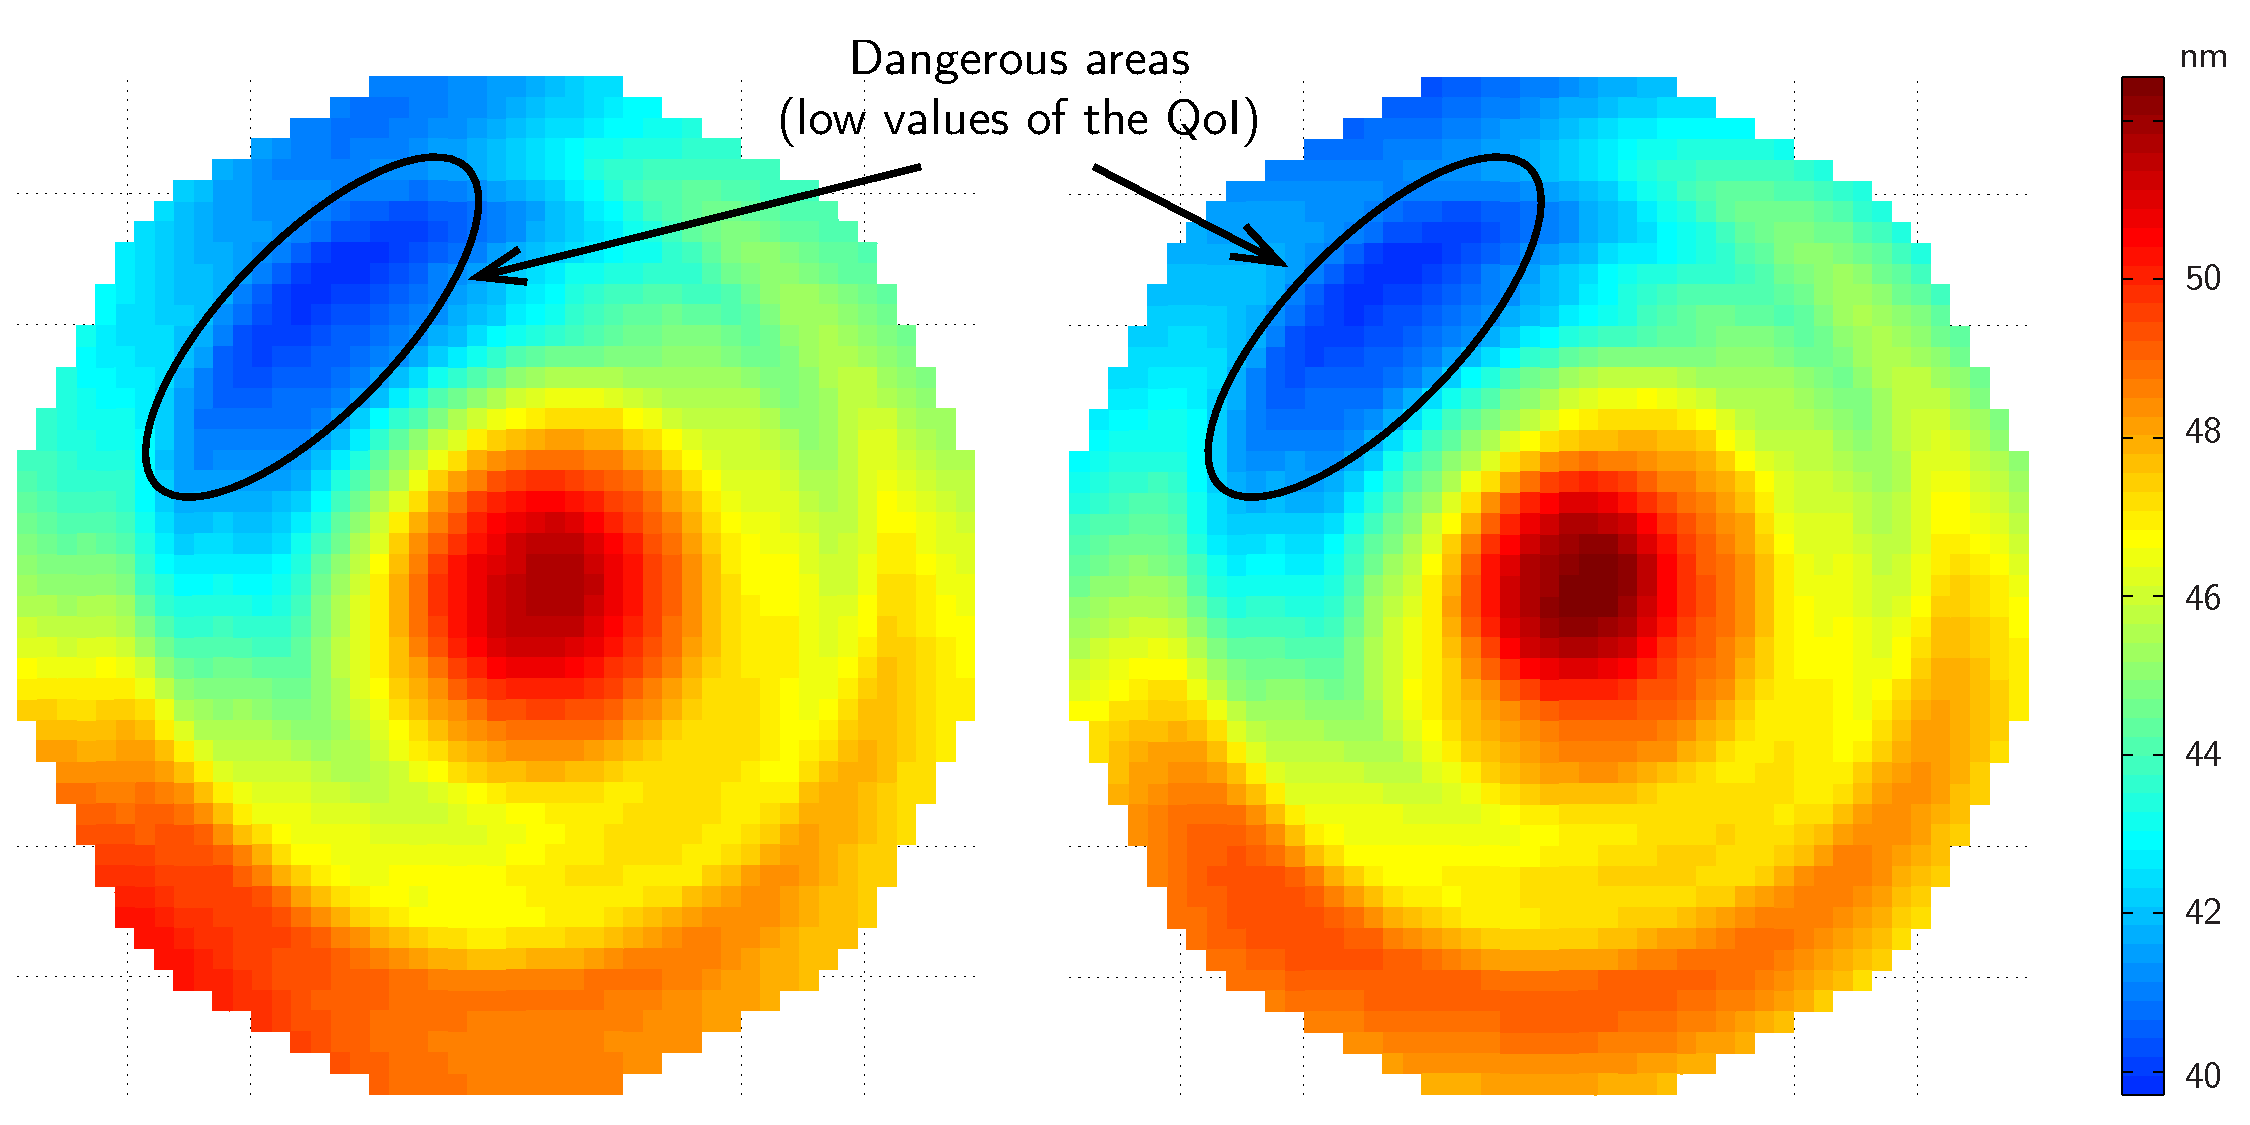
\includegraphics[width=1\linewidth]{include/assets/wafer-qoi.pdf}
  \caption{The true (on the left) and inferred (on the right) distribution of the QoI across the wafer.}
  \flabel{wafer-qoi}
\end{figure}

Let us consider an example that illustrates a particular application of the proposed technique. As previously mentioned, due to process variation, the key parameters that have direct impacts on power and temperature are intrinsically uncertain. Let $\u$ be one of such uncertain quantities; say, the effective channel length. Assume the manufacturing process imposes a lower bound $\u_*$ on the parametrization $\u$. This lower bound separates defective dies ($\u < \u_*$) from those that function properly ($\u_* \leq \u$). Possible actions that one might wish to take with respect to a single die on the wafer are: (a) keep the die if it closely conforms to the specification; (b) throw away the die if it exhibits an unacceptable divergence, due to process variation, from the specification. Let the distribution of $\u$ across the wafer be the one depicted on the left side of \fref{wafer-qoi} where 316 dies, four cores each, are placed in a $20 \times 20$ grid, and the gradient from navy to dark red represents the transition of $\u$ from low to high values.\footnote{The experimental setup is described in \sref{experimental-results} in detail.} A common approach to find this distribution is to deploy adequate test structures on the dies and measure $\u$ directly; then, the corresponding decision can be taken based on the collected information. The problem in this scenario, however, is that the described procedure is typically highly expensive to undertake.

The technique that we propose and develop in this paper operates on cheap, indirect measurements and, therefore, can considerably decrease the above-mentioned costs since no additional on-die test structures are required. The result of our framework applied to a data set, corrupted by noise, corresponding to only 20 spatial locations on the wafer (out of 316) is shown on the right side of \fref{wafer-qoi}. It can be seen that the fields closely match each other; the normalized root-mean-square error (NRMSE) is below $2.8\%$ in this example. Further, the technique can readily be utilized to estimate probabilities of various events, \eg, $\probabilityMeasure(\u < \u_*)$. This fact is especially advantageous since, in reality, we do not know the true values and, therefore, can reason about our decisions only in terms of probabilities. We can then reformulate our decision rule as follows: (a) keep the die if $\probabilityMeasure(\u_* \leq \u)$ is larger then a certain threshold; (b) throw the die away, otherwise. An illustration of this decision process is given in \fref{wafer-defect} where the threshold is set to two standard deviation below the mean value of $\u$, the circles mark defective dies (the navy areas in \fref{wafer-qoi}), and the gradient from light gray to red corresponds to the inferred probability of a die to be defective. It can be seen that the inference accurately detects faulty regions.
\begin{figure}[t!]
  \centering
  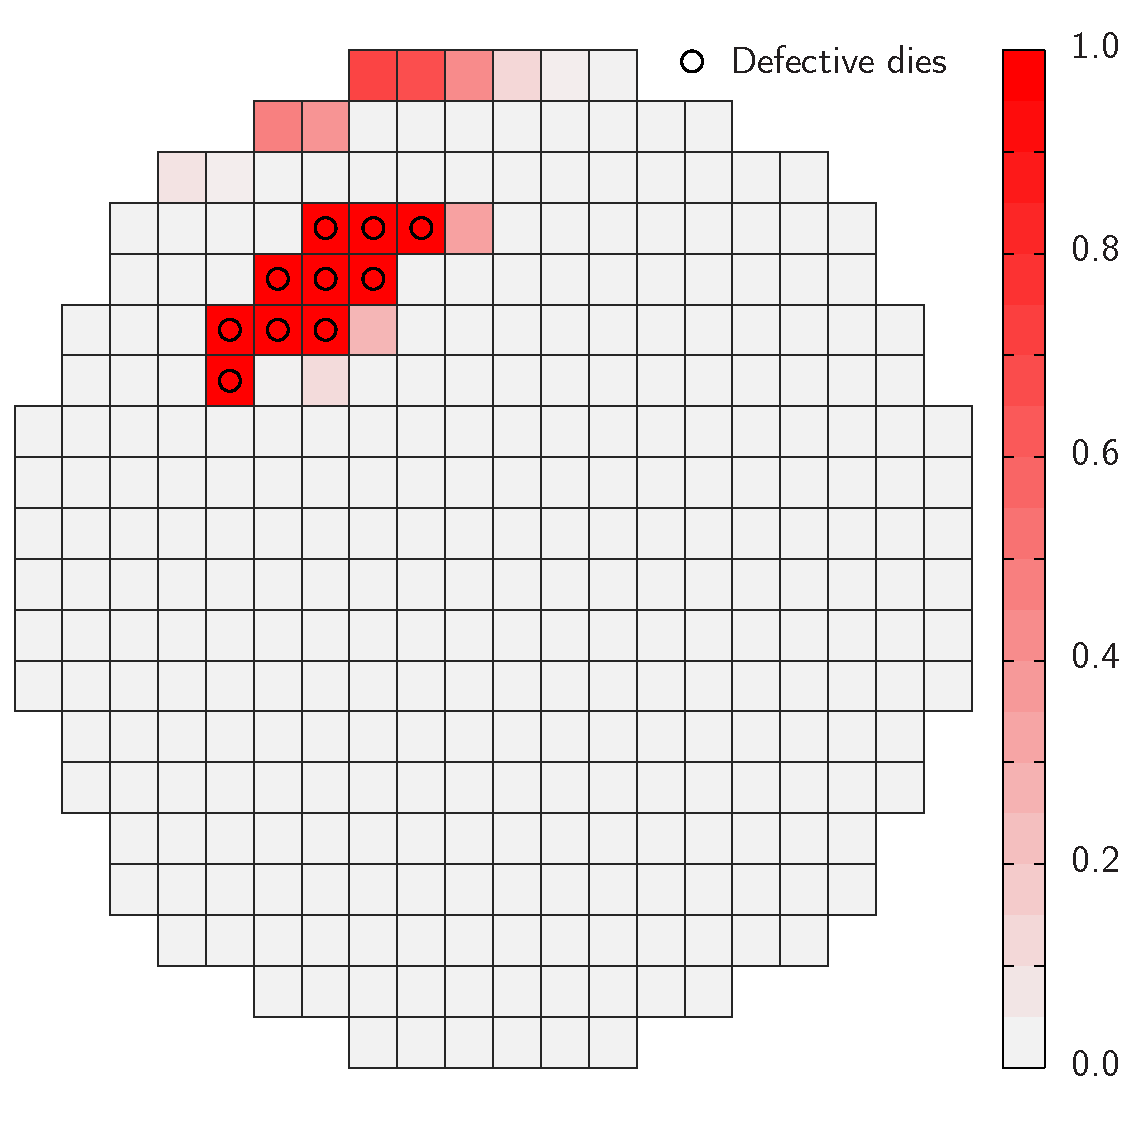
\includegraphics[width=0.7\linewidth]{include/assets/wafer-defect.pdf}
  \caption{Inferred probability of defective dies.}
  \flabel{wafer-defect}
  \vspace{-1.5em}
\end{figure}


In addition, we can introduce a trade-off action: (c) expose the die to a thorough inspection (\eg, via a test structure) if the threshold of (a) is no reached, and (b) has a separate threshold, which is also not satisfied. In this case, we can save money by examining only those dies for which there is no strong evidence of their satisfactory or unsatisfactory condition. Furthermore, one can introduce into play a so-called utility function, which, for each combination of an outcome of $\u$ and a taken action, \ie, (a), (b), and (c) in our example, assigns the corresponding amount of gain that the decision maker receives. Then, the inference path taken in this paper (Bayesian inference) can deliver such an action that maximized the expected utility with respect to the posterior distribution of $\u$; in other words, all possible outcomes of $\u$ weighted by their probabilities will be taken into account in the final decision.


  \section{Problem Formulation} \slabel{problem-formulation}
  Consider an electronic system that consists of $\nprocs$ active components, \ie, those that dissipate power, identified at the intended level of granularity (processors, ALUs, caches, registers, \etc); hereafter, these components are referred to as processing elements.
The system is being produced on a silicon wafer that hosts $\ndies$ dies.
Let $\specification$ be a set of layout-and-temperature-related information including: (a) the floorplan of the wafer, (b) the floorplan of a die on the wafer, and (c) the thermal parameters of the materials that the dies are made of.

A power profile $\profileP$ of a die is a tuple composed of a data matrix $\mP = (\vP_i) \in \real^{\nprocs \times \nsteps}$, $\vP_i \in \real^\nprocs$, that captures the power dissipation of all the $\nprocs$ processing elements at $\nsteps$ moments of time and a (column) vector $\partition{\mP} = (\t_i) \in \real^{\nsteps}$ with positive and strictly increasing components that specifies these moments of time.
The definition of a (transient) temperature profile $\profileT$ is the same as the one for power except that the data matrix $\mT$ contains temperature.

The system is assumed to depend on a random element (such as the effective channel length and gate oxide thickness), denoted by $\u$, which manifests itself in deviations of the actual power dissipation from nominal values and, consequently, in deviations of temperature from the one corresponding to the nominal power consumption. It what follows, $\u$ is referred to as the quantity of interest (\qoi).

The goal of this work is to develop a framework for the characterization of the distribution of $\u$ across the wafer with the following properties: (a) low deployment costs, (b) computational efficiency, (c) ability to operate on incomplete and noisy data, and (d) ability to accommodate the prior knowledge of the user on $\u$.
The inputs to our framework should be composed of (a) a set of layout-and-temperature-related information $\specification$, (b) a workload given as a detailed dynamic power profile $\profilePdyn$, and (c) prior knowledge on $\u$.
The output of the framework should comprise the required by the user statistics about the \qoi.
A graphical representation of the inputs and outputs is given in \fref{algorithm}, which is further described in \sref{proposed-framework}.

To achieve the established goal, we propose the use of indirect measurements.
Specifically, we aim at measuring temperature, which we shall then analyze using Bayesian inference.
Thus, as the first step, the user is supposed to harvest, as described in \sref{motivation}, a set of temperature profiles, corresponding to $\profilePdyn$, at several locations on the wafer.
Denote by $\Data = \{ (\mT^{(i)}_\meas, \partition{\mT}), \r_i \}_{i = 1}^\nrdies$ such a data set composed of $\nrdies$ temperature profiles $(\mT^{(i)}_\meas, \partition{\mT})$ of $\nrdies$ out of $\ndies$ dies on the wafer and the corresponding spatial locations of these dies $\vr = (\r_i) \in \domain^\nrdies$ in the domain $\domain$ representing the surface of the wafer.
It is important to note that $\mT^{(i)}_\meas$ can potentially contain data only for a subset of the processing elements, say $\nrprocs \leq \nprocs$ (see \fref{wafer-measured} for an illustration), and/or only for a subset of the time moments of the power partition $\partition{\mP}$, say $\nrsteps \leq \nsteps$; therefore, $\mT^{(i)}_\meas \in \real^{\nrprocs \times \nrsteps}$.
For simplicity, the temperature profiles in $\Data$ are assumed to share the same subset of the measured processing elements and the same time partition.
This time partition is presumably sparse as it is more practical to track temperature at a much lower frequency than the one used for power, \ie, $\nrsteps \ll \nsteps$.
For the same practical reason, the number of measured dies is presumably much smaller than the total number of dies, \ie, $\nrdies \ll \ndies$, as shown in \fref{wafer-measured}.


  \section{Preliminaries} \slabel{preliminaries}
  \subsection{Bayesian Inference} \slabel{bayesian-inference}
Let $\vparam$ be a set of parameters that are uncertain for us either in nature or due to our limited knowledge. The goal is to characterize the distribution of $\vparam$ given a data set of observations and some prior believes on $\vparam$. A natural solution is to rely on Bayes' rule \cite{gelman2004}:
\begin{equation} \elabel{bayes}
  \text{Prior} = \frac{\text{Likelihood} \times \text{Prior}}{\text{Evidence}}, \;\; \f{\vparam | \Data} = \frac{\f{\Data | \vparam} \f{\vparam}}{\f{\Data}},
\end{equation}
where $\f{\cdot}$ denotes a probability density function, and the straight bars stand for conditioning. $\f{\vparam}$ is called the prior of $\vparam$, $\f{\vparam | \Data}$ is the corresponding posterior, $\f{\Data | \vparam}$ is the likelihood function, and $\f{\Data}$ is a normalization constant. Closed-form expressions for posteriors often do not exist for challenging problems. For instance, when modeling a physical process, the likelihood function may involve solving a system of differential equations; it is the case for our problem as we shall see in \sref{thermal-model}. Thus, in order to be able to draw samples from the posterior, one usually relies on sampling techniques. In this paper, we utilize MCMC sampling \cite{gelman2004}, namely a combination of the Gibbs sampling and the Metropolis algorithm.

\subsection{Karhunen-Lo\`{e}ve (KL) Expansion} \slabel{kl-expansion}
Let $\u: \outcomes \times \domain \to \real$ be a square-integrable stochastic process defined over a spatial domain $\domain$. Let $\fMean{\r} := \E{\u(\r)}$ and $\fCov{\r, \r'} := \E{(\u(\r) - \fMean{\r}) (\u(\r') - \fMean{\r'})}$, $\r, \r' \in \domain$, be the mean and covariance functions of $\u$, respectively. Take a vector of spatial locations $\vr = (\r_i) \in \domain^n$, and define the corresponding discretization of $\u$ as an $n$-dimensional \rv\ $\vu = (\u(\r_i)) \in \real^n$ endowed with the expected value $\vmean = (\fMean{\r_i}) \in \real^n$ and the covariance matrix $\mCov = (\fCov{\r_i, \r_j}) \in \real^{n \times n}$. Since any covariance matrix is real and symmetric, it admits the eigenvalue decomposition \cite{press2007} written as
\[
  \mCov = \m{V} \m{\Lambda} \m{V}^T
\]
where $\m{V}$ and $\m{\Lambda} = \diag{\lambda_i}$ are an orthogonal matrix of the eigenvectors and a diagonal matrix of the eigenvalues of $\mCov$, respectively. Consequently, denoting $\mKL = \m{V} \m{\Lambda}^\frac{1}{2}$, $\vu$ can be represented as
\begin{equation} \elabel{kl-expansion}
  \vu = \vmean + \mKL \vz
\end{equation}
where $\vz$ is a vector of centered, normalized, and uncorrelated \rvs, which are also independent if $\u$ is Gaussian.

The decomposition above provides means of even further model order reduction. The intuition is that, due to the correlations induced by $\fCov$, $\vu$ can be nearly losslessly recovered from a small subset of $\vz$. One way to reveal these redundancies is to analyze the eigenvalues $\lambda_i$ stored in $\m{\Lambda}$. Assume $\lambda_i$, $\forall i$, are arranged in a non-increasing order and let $\tilde{\lambda}_i = \lambda_i / \sum_j \lambda_j$. Gradually summing up the arranged and normalized eigenvalues $\tilde{\lambda}_i$, we can identify a subset of them, which has the cumulative sum greater than a certain threshold. When this threshold is sufficiently high (close to one), the rest of the eigenvalues and their eigenvectors can be dropped as being insignificant, reducing the number of stochastic dimensions. In what follows, such a reduction will have the same notation as in the full version given in \eref{kl-expansion}, and the dimensionality of $\mKL$ and $\vz$ will be clear from the context.

\subsection{Gaussian Process (GP) Regression} \slabel{gp-approximation}
Consider an unknown function $f: \real^\nin \to \real$. We would like to compute $f$ at $\nuno$ unobserved locations $\{ \v{x}_i \}_{i = 1}^\nuno$, $\v{x}_i \in \real^\nin$, based on a set of $\nobs$ observations $\DesignData = \{ (\v{x}_{0i}, y_{0i}) \}_{i = 1}^\nobs$, $\v{x}_{0i} \in \real^\nin$ and $y_{0i} \in \real$. The data are modeled as $y_i = f(\v{x}_i) + \noise_i$ where $\noise_i$ is the noise term. Let $\m{X} = (\v{x}_i) \in \real^{\nin \times \nuno}$, $\m{X}_0 = (\v{x}_{0i}) \in \real^{\nin \times \nobs}$, and $\v{y}_0 = (y_{0i}) \in \real^\nobs$. We put a zero-mean Gaussian process prior on $f$:
\[
  f | \vparam \sim \gaussianp{0}{\fCov},
\]
where $\fCov{\r, \r'} = \E{f(\r) f(\r')}$ is the covariance function of $f$, parametrized by $\vparam$, and a zero-mean Gaussian prior on $\noise_i$:
\[
  \noise_i | \sigma^2_\noise \sim \gaussian{0}{\sigma^2_\noise}.
\]
It can be shown \cite{mackay2003, rasmussen2006} that the corresponding predictive distribution is Gaussian:
\begin{align*}
  & f | \m{X}, \Data \sim \gaussian{\vmean}{\mCov}, \\
  & \vmean = \fCov{\m{X}, \m{X}_0} (\fCov{\m{X}_0, \m{X}_0} + \sigma^2_\noise \mI)^{-1} \v{y}_0, \\
  & \mCov = \fCov{\m{X}, \m{X}} - (\fCov{\m{X}_0, \m{X}_0} + \sigma^2_\noise \mI)^{-1} \fCov{\m{X}_0, \m{X}},
\end{align*}
where, conventionally, the covariance function $\fCov$ applied to two matrices of input variables denotes the matrix obtained by evaluating $\fCov$ on those variables.


  \section{Proposed Framework} \slabel{proposed-framework}
  \begin{figure}
  \centering
  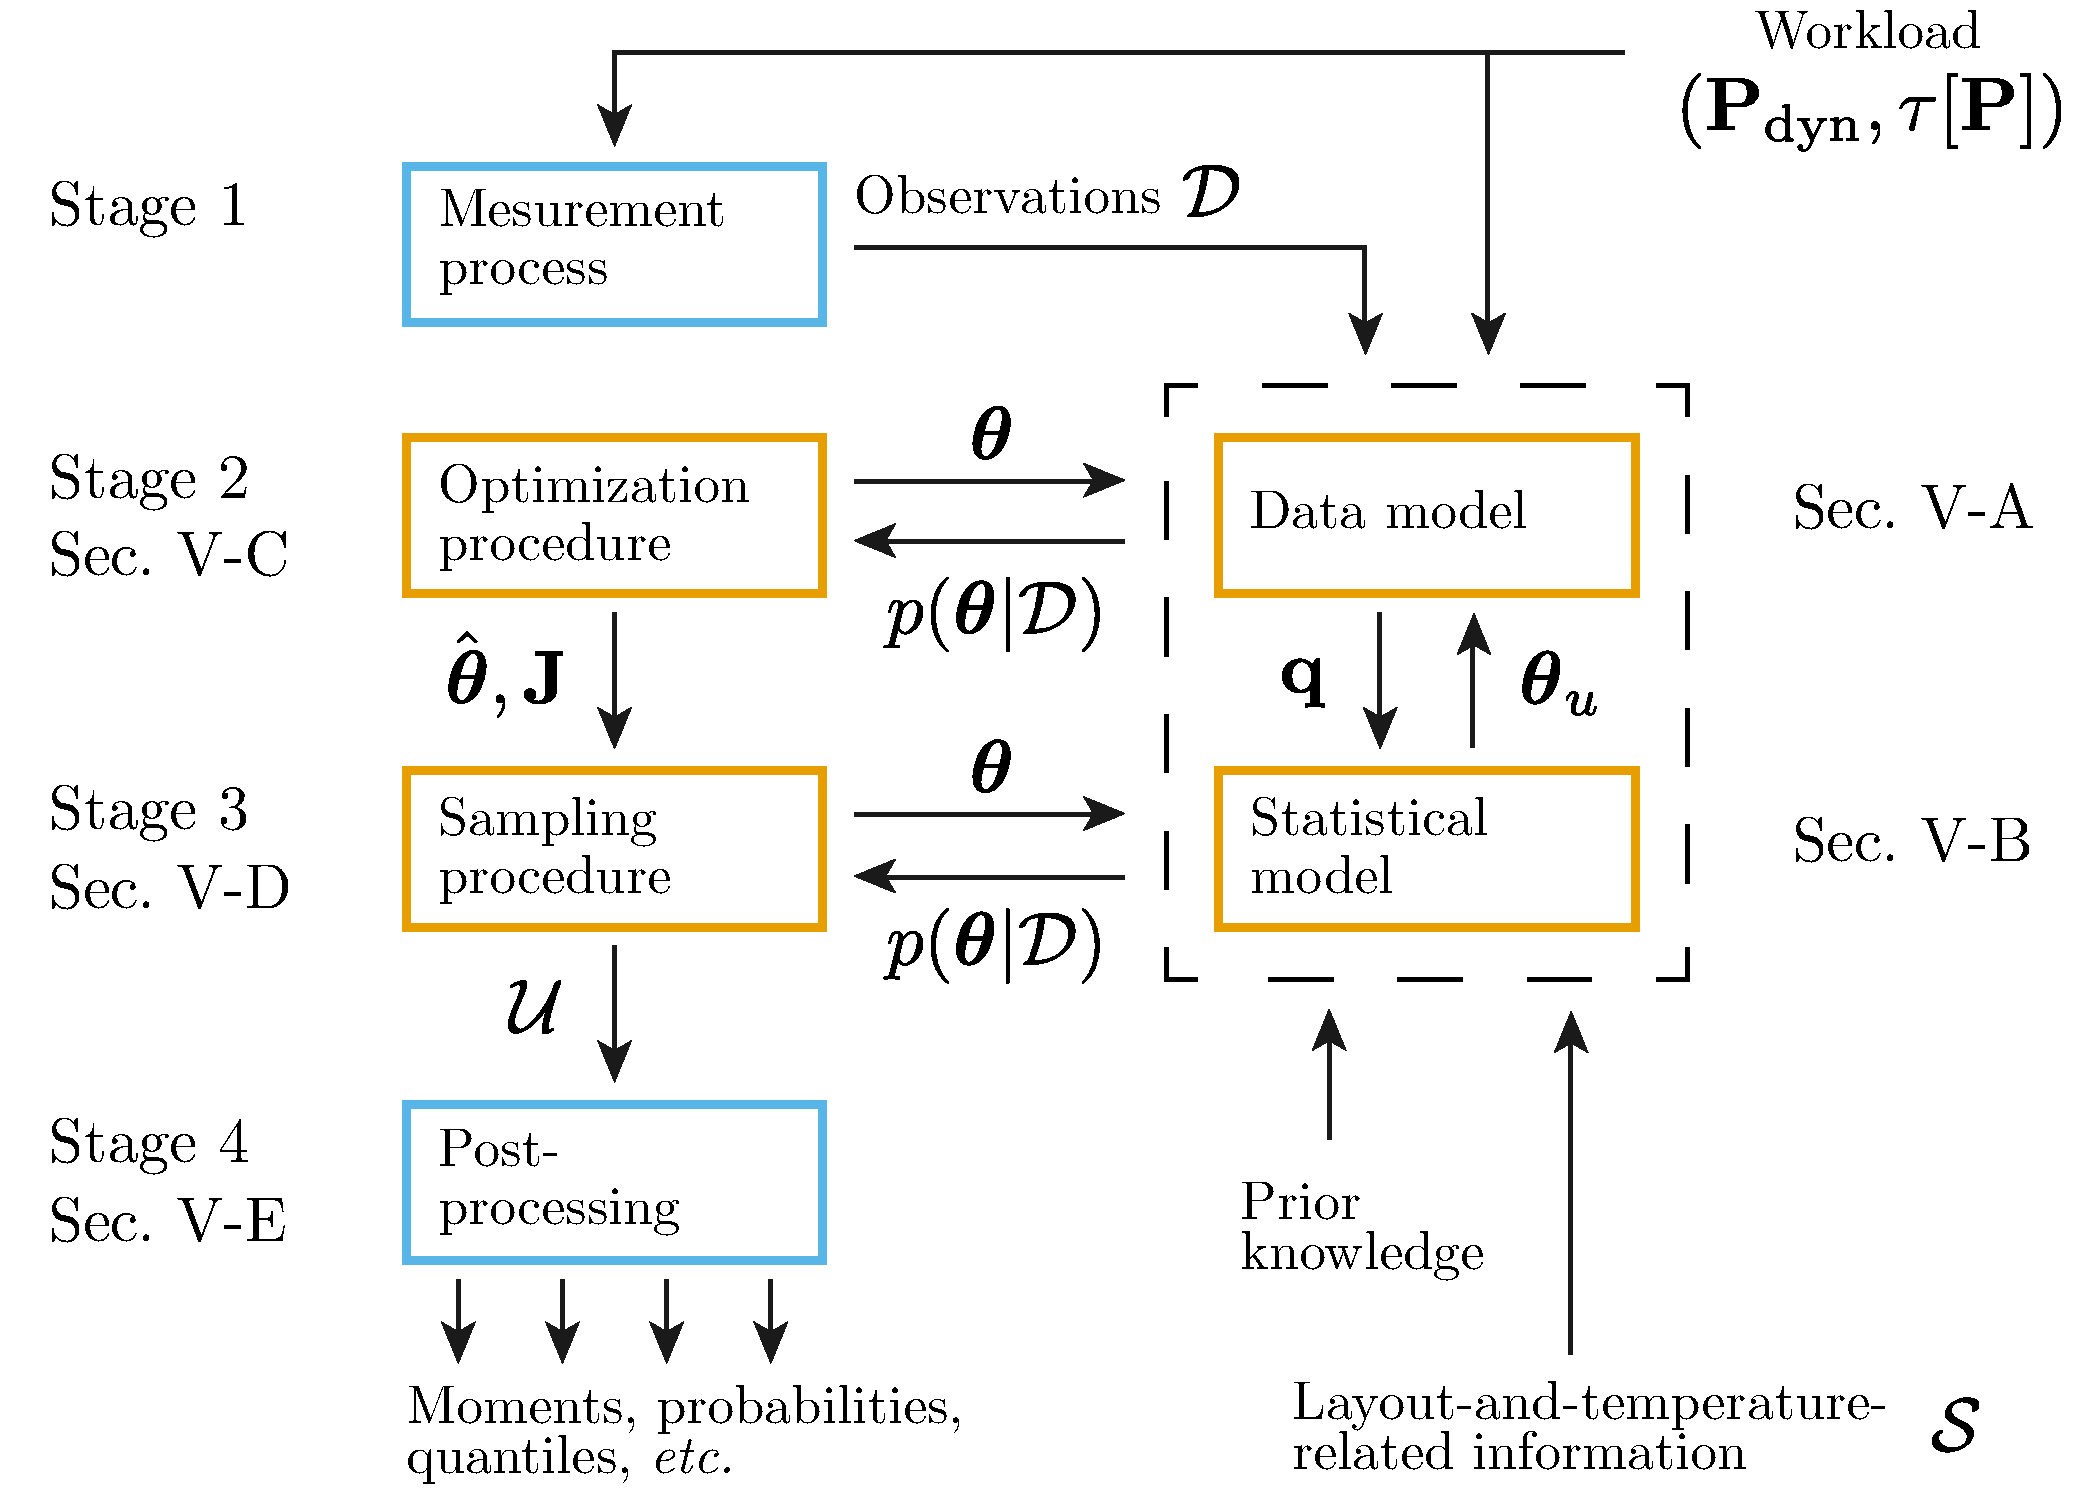
\includegraphics[width=0.80\linewidth]{include/figures/algorithm.pdf}
  \caption{The proposed framework.}
  \flabel{algorithm}
\end{figure}

In this section, we present our temperature-based technique for the characterization of process variation. The framework is divided into four major stages depicted in \fref{algorithm}.
Stage~1 is the data-harvesting stage wherein the user is supposed to collect a set of observations $\Data$ as described in \sref{motivation}.
At Stage~2, we undertake an auxiliary procedure that delivers an optimized proposal distribution to the MCMC sampling in Stage~3.
Stage~3 produces a collection of samples of the \qoi, such as the effective channel length, which is then processed at Stage~4 in order to estimate various characteristics, specified by the user, of this \qoi, \eg, to compute the probability of the effective channel length to be smaller than a certain threshold as motivated in \sref{motivation}.
As it can be seen in \fref{algorithm}, Stage~2 and Stage~3 actively communicate with two models on the right, called the data and statistical models, which we shall discuss next.

\subsection{Data Model} \slabel{data-model} \slabel{power-model} \slabel{thermal-model}
The total power of a system with $\ncores$ processing elements at time $\t$ is composed of the dynamic and leakage parts:
\begin{equation} \elabel{total-power}
  \vP(\t, \vT(\t), \u) = \vP_\dyn(\t) + \vP_\leak(\vT(\t), \u)
\end{equation}
where $\vP, \vT \in \real^\ncores$ are vectors of power and temperature, respectively, and $\u$ is an outcome of the parametrization $\U$. The dynamic part, $\vP_\dyn$, is temperature-independent whereas the leakage part, $\vP_\leak$, is a strong function of the operating temperature. The influence of process variation on the dynamic power is known to be negligibly small \cite{srivastava2010}; therefore, only leakage is assumed to be dependent on $\U$.


Given the thermal specification $\specification$ (see \sref{problem-formulation}) of the multiprocessor system at hand, an equivalent representation, capturing the thermal behavior of the system, can be constructed \cite{kreith2000}. This representation is known as a thermal RC circuit, which is composed of a number of thermal nodes. The structure of the circuit depends on the intended level of granularity and, therefore, impacts the resulting accuracy. For clarity of presentation, we assume that each processing element is mapped onto one corresponding node, and the thermal package is represented as a set of additional nodes. Temperature of the multiprocessor platform is then modeled with the following system of differential-algebraic equations:
\begin{subnumcases}{\elabel{thermal-system}}
  \mC \: \frac{d\vX(\t)}{d\t} + \mG \: \vX(\t) = \mM \: \vP(\t, \vT(\t), \u) \elabel{heat-de} \\
  \vT(\t) = \mM^T \vX(\t) + \vT_\amb \elabel{temperature-output}
\end{subnumcases}
where $\nnodes$ is the number of thermal nodes in the circuit; $\mC \in \real^{\nnodes \times \nnodes}$ is a diagonal matrix of the thermal capacitance; $\mG \in \real^{\nnodes \times \nnodes}$ is a symmetric, positive-definite matrix of the thermal conductance; $\vX \in \real^\nnodes$ is the internal state vector; $\vP \in \real^\nprocs$ and $\mM \in \real^{\nnodes \times \nprocs}$ are the input power vector and its mapping matrix to the thermal nodes; $\vT \in \real^\nprocs$ is the temperature vector, and $\vT_\amb \in \real^\nprocs$ is the vector of the ambient temperature. In general, \eref{heat-de} does not have a closed-form solution due to the power term defined in \eref{total-power}; hence, the system is typically being solved numerically. Consequently, given a dynamic power profile $\profilePdyn$ and using \eref{total-power} and \eref{thermal-system}, we can compute the corresponding temperature profile $(\mT, \partition{\mP})$ where $\mT = (\vT(\t_i))$, $\t_i \in \partition{\mP}$.


\slabel{analytical-solution}
The thermal model above is computationally expensive as it involves a system of nonlinear differential equations (see \eref{heat-de}), which should be solved numerically using, \eg, Runge-Kutta methods \cite{press2007}. In order to mitigate these computations, we utilize the approach discussed in \cite{ukhov2012}.
The idea is that, if the power term on the right-hand side of \eref{heat-de} stays constant, the system becomes linear and has an analytical solution. When the simulated time interval was short enough, the technique was found to have a negligibly small influence on the resulting accuracy; however, the speedup was found to be considerable.
Since $\profilePdyn$ is fine-grained, we can assume that the total power changes only at the time moments $\t_i \in \partition{\mP}$ (see \sref{problem-formulation}). In this way, we can stride in time solving \eref{heat-de} for each step analytically and, thus, gaining a significant speedup.

Now we apply the derivation above to evaluate $\nrdies$ temperature profiles at the locations of the measurements in $\Data$, \ie, at $\{ \r_i \}_{i = 1}^\nrdies$.
The resulting profiles are then shrunk to keep data only for those processing elements and only for those moments of time that are present in the measured temperature profiles, \ie, we keep data only for $\nrprocs$ (out of $\nprocs$) processing elements and only for $\nrsteps$ (out of $\nsteps$) moments of time (see \fref{wafer-measured}).
The trimmed profiles are then stacked into one vector with $\nrdies \nrprocs \nrsteps$ elements, which is denoted by $\mvT$.
In what follows, we refer to the overall procedure, starting from power and yielding the temperature vector $\mvT$, as the data model (see \fref{algorithm}).
Also, let $\mvT_\meas \in \real^{\nrdies \nrprocs \nrsteps}$ be the stacked version of the data in $\Data$, preserving the one-to-one spatial correspondence between the respective elements of $\mvT$ and $\mvT_\meas$.


\subsection{Statistical Model} \slabel{statistical-model}
Since, at each point of the continuum of spatial locations on the wafer, the random element $\u$ can potentially take a different value, $\u$ is infinite-dimensional.
We model $\u$ as a square-integrable stochastic process $\u: \outcomes \times \domain \to \real$ defined over a spatial domain $\domain$ (see also \aref{kl-expansion}), which corresponds to the wafer.
Uncertainties due to process variation are known to be well approximated using Gaussian distributions \cite{srivastava2010}; therefore, $\u$ is assumed to be a Gaussian process \cite{rasmussen2006}:
\[
  \u | \vparam_\u \sim \gaussianp{\fMean}{\fCov}
\]
where $\fMean$ and $\fCov$ are the mean and covariance functions of $\u$, and $\vparam_\u$ denotes their parametrization. For simplicity, let $\fMean{\r} = \mu$, $\forall \r \in \domain$, meaning that the expected value is constant.
$\fCov$ is chosen to be the following composition:
\begin{equation} \elabel{covariance-function}
  \fCov{\r, \r'} = \sigma_\u^2 \big( \eta \fCov_\SE(\r, \r') + (1 - \eta) \fCov_\OU(\r, \r') \big)
\end{equation}
where
\begin{align*}
  & \fCov_\SE(\r, \r') = \exp\left(-\frac{\norm{\r - \r'}^2}{\ell_\SE^2}\right) \text{ and} \\
  & \fCov_\OU(\r, \r') = \exp\left(- \frac{\abs{\,\norm{\r} - \norm{\r'}\,}}{\ell_\OU} \right)
\end{align*}
are the squared exponential and Ornstein-Uhlenbeck kernels, respectively; $\sigma_\u^2$ represents the variance of $\u$; $\eta \in [0, 1]$ weights the kernels; $\ell_\SE$ and $\ell_\OU > 0$ are the length-scale parameters; $\norm{\cdot}$ stands for the Euclidean distance.
The choice of the covariance function is guided by the observations of the correlation structures induced by the manufacturing process \cite{cheng2011}: the first kernel, $\fCov_\SE$, imposes similarities between the points on the wafer that are close to each other while the second kernel, $\fCov_\OU$, imposes similarities between points that are at the same distance from the center of the wafer.
In this work, $\eta$, $\ell_\SE$, and $\ell_\OU$ are assumed to be given while $\mu$ and $\sigma^2_\u$ are a part of our inference. Thus, we let $\vparam_\u = \{ \mu, \sigma_\u^2 \}$.

\subsubsection{Model order reduction} \slabel{model-order-reduction}
The infinite-dimensional object $\u$ is reduced to a finite-dimensional one via the Karhunen-Lo\`{e}ve (KL) expansion introduced in \aref{kl-expansion}. The discretization is performed with respect to the spatial locations of all $\ncp = \nchips \nprocs$ processing elements on the wafer. Consequently, we obtain an $\ncp$-dimensional \rv\ denoted by $\vu: \outcomes \to \real^\ncp$:
\begin{equation} \elabel{kl-approximation}
  \vu = \mu \vI + \sigma_\u \mKL \vz
\end{equation}
where we treat the constant multiplier $\sigma^2_\u$ in \eref{covariance-function} separately, $\vz = (\z_i) \in \real^\nvars$ obey the standard Gaussian distribution, and $\vI = (e_i = 1)$. Note that model order reduction (see \aref{kl-expansion}) is implied in \eref{kl-approximation}; thus, $\vz \in \real^\nvars$ where $\nvars \leq \ncp$. In addition, we denote by $\vu_\data \in \real^{\ndp}$, $\ndp = \ndata \nprocs$, those elements of $\vu$ that correspond to the observations in $\Data$. Let us redefine $\vparam_\u = \{ \vz, \mu, \sigma^2_\u \}$ and denote the forward model by $\model{\vparam_\u}$.

\subsubsection{The likelihood function}
Due to the imperfection of the measurement process, the temperature profiles in $\Data$, stacked into $\mvT_\meas$, are assumed to deviate from the model prediction in \eref{model}. To account for this,
\[
  \mvT_\meas = \model{\vparam_\u} + \vnoise = \mvT + \vnoise
\]
where $\vnoise$ is an $\ndps$-dimensional vector of noise. The noise is typically assumed to be a white Gaussian noise and to be independent of $\u$ \cite{rasmussen2006, marzouk2009}. Therefore,
\[
  \vnoise | \sigma^2_\noise \sim \gaussian{0}{\sigma^2_\noise \mI}
\]
where $\sigma^2_\noise$ is a parameter defining the variance of the noise; imposing no loss of generality, the noise is assumed to have the same magnitude for all measurements. The measurement noise can be interpreted as
\begin{equation} \elabel{likelihood}
  \mvT_\meas | \vparam_\u, \sigma_\noise^2 \sim \gaussian{\mvT}{\sigma_\noise^2 \mI}
\end{equation}
yielding the likelihood function of the data $\Data$.

\subsubsection{The prior}
Denote the parameters to be inferred as
\[
  \vparam = \vparam_\u \cup \{ \sigma_\noise^2 \} = \{ \vz, \mu, \sigma_\u^2, \sigma_\noise^2 \}.
\]
We put the following priors on $\vparam$:
\begin{align}
  & \z_i \sim \gaussian{0}{1}, \elabel{z-prior} \\
  & \mu \sim \gaussian{\mu_0}{\sigma^2_0}, \elabel{mu-u-prior} \\
  & \sigma^2_\u \sim \sichisquared{\nu_\u}{\tau^2_\u}, \text{ and} \elabel{sigma2-u-prior} \\
  & \sigma^2_\noise \sim \sichisquared{\nu_\noise}{\tau^2_\noise}. \elabel{sigma2-noise-prior}
\end{align}
The prior for $\vz$ is due to the properties of the KL expansion. The next three priors, \ie, a Gaussian and two scaled inverse chi-squared distributions, are a common choice for a Gaussian model with the mean and variance being unknown \cite{gelman2004}. The hyperparameters $\mu_0$, $\tau_\u$, and $\tau_\u$ represent the presumable values of $\mu_u$, $\sigma_\u$, and $\sigma_\noise$, respectively, and the hyperparameters $\sigma_0$, $\nu_\u$, and $\nu_\noise$ reflect the degree of our beliefs according to our prior knowledge. In the absence of such knowledge, non-informative priors can be chosen (see, \eg, \cite{gelman2004}).

\subsubsection{The posterior}
Taking the product of the likelihood in \eref{likelihood} and the priors in \eref{z-prior}--\eref{sigma2-noise-prior}, we obtain
\begin{align}
  & \ln \f{\vparam | \Data} + c = -\frac{\ndps}{2} \ln \sigma^2_\noise - \frac{\norm{\mvT_\meas - \mvT}^2}{2 \sigma^2_\noise} \nonumber \\
  & {} - \frac{\norm{\vz}^2}{2} - \frac{(\mu - \mu_0)^2}{2 \sigma^2_0} - \left(1 + \frac{\nu_\u}{2}\right) \ln \sigma^2_\u - \frac{\nu_\u \tau_\u^2}{2 \sigma^2_\u} \nonumber \\
  & {} - \left(1 + \frac{\nu_\noise}{2}\right) \ln \sigma^2_\noise - \frac{\nu_\noise \tau_\noise^2}{2 \sigma^2_\noise} \elabel{log-posterior}
\end{align}
where $c$ is some constant. This expression is sufficient for the Metropolis algorithm (see \aref{bayesian-inference}); thus, we can readily draw samples from the posterior. Each sample of $\vparam_\u$ is then used in \eref{kl-approximation} to compute a sample of $\u$, \ie, the QoI that we are concerned with, for all processing elements on the wafer.
Note, however, the likelihood function poses a significant computational challenge as each sample requires an evaluation of $\model$; we shall address this issue in \sref{computational-aspects}.


\subsection{Optimization of the Proposal Distribution} \slabel{optimization}
In this section, we describe the objective of Stage~2 in \fref{algorithm}.
The core of the Metropolis-Hastings algorithm is the proposal distribution (see \sref{bayesian-inference}) as a carefully constructed proposal can significantly reduce the number of steps needed for obtaining a good approximation of the posterior distribution; in other words, it can save a lot of evaluations of $\model$.
A common technique to construct a high-quality proposal is to perform an optimization procedure of the log-posterior given by \eref{log-posterior}; more specifically, one seeks for such $\vparam$ that maximizes \eref{log-posterior}.
By doing so, we obtain the most probable value of $\vparam$, called the posterior mode and denoted by $\hat{\vparam}$, and also compute the negative of the Hessian matrix at $\hat{\vparam}$, called the observed information matrix and denoted by $\mOI$. The two form a solid base for the proposal.
For example, a classical proposal is a multivariate Gaussian distribution wherein the mean is the current location of the chain, and the covariance matrix is the inverse of $\mOI$; see \cite{gelman2004, bernardo2007}.


\subsection{Sampling via the Metropolis-Hastings Algorithm} \slabel{sampling}
Let us turn to the sampling stage, Stage~3 in \fref{algorithm}. As mentioned earlier, we utilize the Metropolis algorithm for sampling. In order to speed up this process, we would like to make use of the omnipresent multicore parallelization for sampling. To this end, instead of utilizing the classical proposal mentioned in \sref{optimization}---which is purely sequential as the mean for the next sample draw is dependent on the previous sample---we appeal to a variation of the Metropolis algorithm called the independence sampler Metropolis algorithm \cite{gelman2004}. In this case, a typical choice of the proposal is a multivariate t-distribution, independent of the current position of the chain:
\begin{equation} \elabel{proposal}
  \vparam \sim \studentst{\nu}{\hat{\vparam}}{\alpha^2 \mOI^{-1}}
\end{equation}
where $\hat{\vparam}$ and $\mOI$ are as in \sref{optimization}, $\nu$ is the number of degrees of freedom, and $\alpha$ is a tuning constant. Now, the posterior in \eref{log-posterior} can be computed for all samples in parallel.

Having completed the sampling procedure, we obtain a collection of samples of the parametrization $\vparam$. Since it can take time for a Markov chain to reach regions of high probability (see \sref{bayesian-inference}), a certain number of initial samples are typically discarded as being unrepresentative, which is known as a burn-in period.
Each of the preserved samples of $\vparam$ is then used in \eref{kl-approximation} to compute a sample of $\u$, $\u_i \in \real^{\ndies \nprocs}$.
Denote such a data set with $\nsamples$ samples by $\UData = \{ \u_i \}_{i = 1}^\nsamples$.


\subsection{Post-processing} \slabel{post-processing}
At Stage~4 in \fref{algorithm}, using the set of samples $\UData$, the user computes the desired statistics about the \qoi\ such as the most probable value of the effective channel length at an arbitrary point on the wafer, the probability of an area on the wafer to be defective, \etc\ The computations boil down to the estimation of expected values with respect to the posterior distribution of $\vparam$. This estimation is done in the standard sample-based fashion, that is, in order to compute the expected value of some quantity $h$, one needs to evaluate $h$ for each $\vu_i$ in $\UData$ and then take the average value:
\[
  \E_{\vparam | \Data}(h(\u)) = \int h(\u) \f{\vparam | \Data} d\vparam \approx \frac{1}{\nsamples} \sum_{i = 1}^\nsamples h(\vu_i).
\]
It is worth emphasizing that such statistics can be estimated not only for $\u$ itself, but also for other quantities dependent on $\u$.
For example, we can revert the inference and, given an arbitrary dynamic power profile (different from the one used to collect $\Data$), reason about the corresponding power and temperature profiles, \eg, find the probability density function of the maximal values.
Also, the strength of the Bayesian approach to inference really starts to shine when one needs to take a decision of some kind based on the collected observations in $\Data$; recall the discussion in \sref{motivation}.



  \section{Experimental Results} \slabel{experimental-results}
  \newcommand{\spaceTables}{\hspace{0.5em}}
\begin{table*}
\scriptsize
\begin{minipage}{0.36\linewidth}
  \centering
  \caption{Measured sites \textnormal{$\nrdies$}}
  \begin{tabular*}{1\linewidth}{=l-r-r-r-r-r}
    \toprule
    & 10 & 20 & 40 & 80 & 160 \\
    \midrule
    \midrule
    Optimization time, m & 2.49 & 3.34 &  4.59 &  7.33 & 10.29 \\
    \midrule
    \rowstyle{\bfseries}
    Sequential time, m   & 3.99 & 4.60 &  5.79 &  8.49 & 12.96 \\
    Total time, m        & 6.47 & 7.94 & 10.38 & 15.81 & 23.25 \\
    \midrule
    Parallel time, m     & 1.02 & 1.18 &  1.51 &  2.16 &  3.62 \\
    Total time, m        & 3.50 & 4.52 &  6.10 &  9.49 & 13.91 \\
    \midrule
    NRMSE, \%            & 4.40 & 3.42 &  1.09 &  0.85 &  0.67 \\
    \bottomrule
  \end{tabular*}
  \tlabel{spatial-measurements}
\end{minipage}
\spaceTables
\begin{minipage}{0.23\linewidth}
  \centering
  \caption{Measured points per site \textnormal{$\nprocs$}}
  \begin{tabular*}{1\linewidth}{=r-r-r-r-r}
    \toprule
    2 & 4 & 8 & 16 & 32 \\
    \midrule
    \midrule
    2.67 & 3.34 &  5.20 &  7.37 & 13.85 \\
    \midrule
    \rowstyle{\bfseries}
    3.71 & 4.60 &  6.03 &  8.92 & 14.77 \\
    6.38 & 7.94 & 11.23 & 16.29 & 28.62 \\
    \midrule
    0.98 & 1.18 &  1.58 &  2.51 &  5.30 \\
    3.65 & 4.52 &  6.78 &  9.88 & 19.15 \\
    \midrule
    4.71 & 3.42 &  3.68 &  2.73 &  1.94 \\
    \bottomrule
  \end{tabular*}
  \tlabel{processing-elements}
\end{minipage}
\spaceTables
\begin{minipage}{0.21\linewidth}
  \centering
  \caption{Data amount per point \textnormal{$\nsteps$}}
  \begin{tabular*}{1\linewidth}{=r-r-r-r-r}
    \toprule
    10 & 20 & 40 & 80 & 160 \\
    \midrule
    \midrule
    3.02 & 3.34 & 3.62 & 3.64 & 4.20 \\
    \midrule
    \rowstyle{\bfseries}
    4.38 & 4.60 & 4.67 & 4.80 & 4.97 \\
    7.40 & 7.94 & 8.29 & 8.44 & 9.16 \\
    \midrule
    1.13 & 1.18 & 1.22 & 1.25 & 1.30 \\
    4.16 & 4.52 & 4.84 & 4.89 & 5.50 \\
    \midrule
    2.72 & 3.42 & 1.83 & 2.34 & 1.32 \\
    \bottomrule
  \end{tabular*}
  \tlabel{temporal-measurements}
\end{minipage}
\spaceTables
\begin{minipage}{0.17\linewidth}
  \centering
  \caption{Noise deviation \textnormal{$\sigma_\noise$}}
  \begin{tabular*}{1\linewidth}{=r-r-r-r}
    \toprule
    0~K & 0.5~K & 1~K & 2~K \\
    \midrule
    \midrule
    5.08 & 3.73 & 3.34 & 3.19 \\
    \midrule
    \rowstyle{\bfseries}
    4.76 & 4.70 & 4.60 & 4.71 \\
    9.84 & 8.43 & 7.94 & 7.90 \\
    \midrule
    1.19 & 1.17 & 1.18 & 1.18 \\
    6.27 & 4.91 & 4.52 & 4.37 \\
    \midrule
    0.02 & 2.71 & 3.42 & 4.05 \\
    \bottomrule
  \end{tabular*}
  \tlabel{noise-deviation}
\end{minipage}
\vspace{-1.5em}
\end{table*}

In this section, we assess the proposed framework using the illustrative example carried through the paper: the characterization of the distribution of the effective channel length $\u$ based on temperature profiles $\q$.
This choice of $\u$ and $\q$ for illustration is dictated by the fact that such a high-level parameter as temperature constitutes a challenging task for the inference of such a low-level parameter as the effective channel length, which implies an intense assessment of the propose technique.
In addition, the chosen process parameter is an important target \perse\ as it is affected by process variation the most and considerably impacts the power/heat dissipation \cite{chandrakasan2001, srivastava2010, juan2012}; in particular, it also influence other process-related characteristics such as the threshold voltage.
The performance of our framework is expected to increase when the auxiliary parameter $\q$ resides ``closer'' to the target parameter $\u$ with respect to the transformation $\q = \oBB{\u}$ (see \sref{data-model}) provided that the amount and granularity of the measurement data stay the same.
For instance, such a ``closer'' quantity $\q$ can be the leakage current, which, however, might not always be the most preferable parameter to work with.

Now we shall describe the default configuration of our setup, which, in the following subsections, will be adjusted according to the purpose of each particular experiment.
We consider a 45-nanometer technological process. The diameter of the wafer is 20 dies, the total number of dies $\ndies$ is 316, and the number of processing elements $\nprocs$ in each of the dies is four.
The number of measured dies $\nrdies$ is 20, and these dies are chosen by an algorithm, which pursues an even coverage of the wafer.
The floorplans of the multiprocessor platforms are constructed in such a way that the processing elements form regular grids.
The dynamic power profiles involved in the experiments are based on simulations of randomly generated task graphs.
The sampling interval of these profiles is 1~ms.
The leakage model, parametrized by temperature and the effective channel length, is constructed by fitting to a data set of SPICE simulations of a reference electrical circuit.
The temperature calculations are undertaken using the approach described in \cite{ukhov2012}, which is based on HotSpot v5.02 \cite{hotspot}.\footnote{The floorplans of the platforms, task graphs of the applications, thermal configuration of HotSpot, \etc\ are available online at \cite{sources}.}
The input data set of measurements $\UData$ is obtained as follows: (a) draw a sample of $\u$ from a Gaussian distribution with mean 45~nm and the covariance function given by \eref{covariance-function} wherein the standard deviation is 5\% \cite{juan2012}; (b) perform one temperature simulation per each of the $\nrdies$ selected dies under the corresponding dynamic power profile; (c) shrink the fine-grained temperature profiles to keep only $\nrsteps$, which is equal to 20 by default, evenly spaced moments of time; and (d) perturb the obtained data set using a white Gaussian noise with the standard deviation of $1~\text{K}$ (Kelvin).

Let us turn to the statistical model in \sref{statistical-model} and summarize the intuition and our assignment for each parameter of this model.
In the covariance function given by \eref{covariance-function}, the weight parameter $\eta$ and the two length-scale parameters $\ell_\SE$ and $\ell_\OU$ should be set according to the correlation patterns typical for the production process at hand \cite{chandrakasan2001, cheng2011}; we set $\eta$ to 0.7 and $\ell_\SE$ and $\ell_\OU$ to half the radius of the wafer.
The threshold parameter of the model order reduction procedure described in \sref{model-order-reduction} and utilized in \eref{kl-approximation} should be set high enough to preserve a sufficiently large portion of the variance of the data and, thus, to keep the corresponding results accurate; we set it to 0.99 preserving 99\% of this variance. The resulting dimensionality $\nvars$ of $\vz$ in \eref{kl-approximation} was found to be 27--28.
The parameters $\mu_0$ and $\tau_\u$ of the priors in \eref{priors} are specific to the considered technological process; we set $\mu_0$ to $45~\text{nm}$ and $\tau_\u$ to 5\% of $\mu_0$ \cite{juan2012}.
The parameters $\sigma_0$ and $\nu_\u$ determine the precision of the information on $\mu_0$ and $\tau_\u$ and are set according to the beliefs of the user; we set $\sigma_0$ to 1\% of $\mu_0$ and $\nu_\u$ to ten.
The latter can be thought of as the number of imaginary observations that the choice of $\tau_\u$ is based on.
The parameter $\tau_\noise$ represents the precision (deviation) of the equipments utilized to collect the temperature measurements in the data set $\QData$ and can be found in the technical specification of these equipments; we set $\tau_\noise$ to $1~\text{K}$. The parameter $\nu_\noise$ has the same interpretation as $\nu_\u$; we set it to ten as well.
In \eref{proposal}, $\nu$ and $\alpha$ are tuning parameters, which can be configured based on experiments; we set $\nu$ to eight and $\alpha$ to 0.5.
The number of sample draws is another tuning parameter, which we set to $10^4$; the first half of these samples is ascribed to the burn-in period leaving $5 \cdot 10^3$ effective samples $\nsamples$.
For the optimization in \sref{optimization}, we use the Quasi-Newton algorithm \cite{press2007}.
For parallel computations, we utilize four processors.
Finally, all the experiments are conducted on a GNU/Linux machine with Intel Core i7 2.66~GHz and 8~GB of RAM.

\subsection{Analysis of the Experimental Setup}
In order to ensure that the experimental setup is adequate, let us first perform a detailed analysis of the results obtained for one particular example with the default configuration.
The true and inferred distributions of the \qoi\ are shown in \fref{wafer-qoi} where the normalized root-mean-square error (NRMSE) is below 2.8\%, and the absolute error is bounded by 1.4~nm, which suggests that the framework produces a close match to the true value of the \qoi.
Next we inspect the trace of the obtained sequence of samples and observe that the constructed Markov chain vividly explores the underlying probability space.
Another test commonly used to assess the quality of the proposal distribution is to compare the posterior in \eref{posterior} with the tailored proposal distribution in \eref{proposal} for each parameter conditioned on the other parameters being at $\hat{\vparam}$ (see \sref{optimization}).
The two are found to be practically indistinguishable implying a high quality of the proposal.
To sum up, the performed analysis suggests that the optimization and sampling procedures are tuned well.
In what follows, we shall use the assessed default configuration and alter only one parameter at a time: the number of processing elements on a die $\nprocs$, the number of measured dies on the wafer $\nrdies$, the number of temporal measurements $\nrsteps$, and the deviation of the noise $\sigma_\noise$.

\subsection{Number of Processing Elements on a Die}
In this subsection, we consider five platforms with the number of processing elements in each die $\nprocs$ equal to 2, 4, 8, 16, and 32, respectively. The results are summarized in \tref{processing-elements}.
In this and the following tables, we report the optimization (\stage{2}\ in \fref{algorithm}) and sampling (\stage{3}\ in \fref{algorithm}) times separately (given in minutes); moreover, the sampling time is given for two cases: sequential and parallel computing, which is followed by the total time and error (NRMSE).
The computational time of the post-processing phase (\stage{4}\ in \fref{algorithm}) is not given as it is negligibly small.
The sequential sampling time is the most representative indicator of the computational complexity scaling as the number of samples is always fixed, and there is no parallelization; thus, we shall watch this value in most of the discussions below (highlighted in bold).

It can be seen in \tref{processing-elements} that all computational times grow with the number of processing elements.
This behavior is expected as each processing element increases the amount of work for the temperature simulator.
Nevertheless, even for large examples, the timing is readily acceptable, taking into account the complexity of the inference procedure behind and the yielded accuracy.
An interesting observation can be made from the NRMSE: the error tends to decrease as $\nprocs$ grows.
The explanation is that, with each processing element, $\QData$ delivers more information to the inference to work with since the temperature profiles are collected for all processing elements simultaneously; in our scenario, $\nrprocs = \nprocs$ (\sref{model-order-reduction}).

\subsection{Number of Spatial Measurements}
Let us change the number of dies $\nrdies$ for which the measurement data are available in the input data set $\QData$ (correspondingly, $\ndies - \nrdies$ dies are left unobserved in \fref{wafer-measured}). The considered scenarios are 1, 10, 20, 40, 80, and 160 measured dies, respectively. The results are reported in \tref{spatial-measurements}.
We see that the more data the proposed framework needs to process, the longer the execution time, which is reasonable. The trend, however, is not as steep as the one in \tref{processing-elements} since the thermal system stays unchanged.
The error firmly decreases and drops below 4\% with around 20 measurement points, which is only 6.3\% of the total number of dies on the wafer.

\subsection{Number of Temporal Measurements}
In this subsection, we sweep the number of moments of time $\nrsteps$ for which the measurement data are available in $\QData$. The scenarios are 1, 10, 20, 40, 80, and 160 time moments, respectively. The results are aggregated in \tref{temporal-measurements}.
As we see, the growth of the computational time is relatively small. One might have expected this time to be the same as the one for the spatial measurements since, formally, their influence on the dimensionality of $\QData$ is identical (recall $\vq^\meas \in \real^{\nrdies \nrprocs \nrsteps}$). However, the meaning of the two numbers, $\nrdies$ and $\nrsteps$, is completely different, and, therefore, the way they manifest themselves in the algorithm is also different. Thus, the corresponding amounts of extra data are being treated differently leading to the discordant timing shown in \tref{spatial-measurements} and \tref{temporal-measurements}.
The NRMSE in \tref{temporal-measurements} has a decreasing trend; however, this trend is less steady than the ones discovered before. The finding can be explained as follows. The distribution of the time moments in $\QData$ changes since these moments are kept evenly spaced across the corresponding time spans of the input power profiles.
Some moments of time can be more informative than the other.
Hence, more or less representative samples can end up in $\QData$ helping or misleading the inference.
Based on \tref{spatial-measurements} and \tref{temporal-measurements}, we can also conclude that a larger number of spatial measurements is more advantageous for the inference than a larger number of temporal measurements.

\subsection{Deviation of the Measurement Noise}
Next we vary the standard deviation of the noise (in Kelvins), affecting the data $\QData$, within the set $\{ 0, 0.5, 1, 2 \}$ coherent with the literature \cite{mesa-martinez2007}. Note that the corresponding prior distribution in \eref{priors} is kept unchanged. The results are given in \tref{noise-deviation}.
The sampling time is approximately constant. However, we observe an increase of the optimization time with the decrease of the noise level, which can be ascribed to wider possibilities of perfection for the optimization procedure.
A more important observation, revealed by this experiment, is that, in spite of the fact that the inference operates on indirect and drastically incomplete data, a thoroughly calibrated equipment can considerably improve the quality of predictions.
However, even with a high level of noise of two degrees---meaning that measurements are dispersed over a wide band of 8~K with a large probability of more than 0.95---the NRMSE is still only 4\%.

\subsection{Sequential vs. Parallel Sampling}
Let us summarize the results of the sequential and parallel sampling strategies.
In the sequential MH algorithm, the optimization time is typically smaller than the time needed for drawing posterior samples.
The situation changes when parallel computing is utilized. With four parallel processors, the sampling time decreases 3.81 times on average, which indicates good parallelization properties of the chosen sampling strategy.
The overall speedup ranges from 1.49 to 2.75 with the average value of 1.77 times, which can be pushed even further employing more parallel processors.


  \section{Conclusion} \slabel{conclusion}
  In this paper, we proposed a framework for the analysis of process variation across semiconductor wafers, which is based on cost-efficient indirect measurements analyzed via Bayesian inference.
The technique was exposed to an extensive study of various aspects concerning its implementation.
The obtained results support the computational efficiency and accuracy of our approach.

We would like to note that, although the framework was demonstrated on the effective channel length, it can be readily utilized to analyze any other \qois\ and, moreover, to study their combinations.
In addition, the user is free to replace the data model described in \sref{data-model} with another model, serving the same purpose, if this change is considered to be more beneficial in a different context.


  \printbibliography
\end{document}

% vim: ft=tex
